\documentclass[xcolor=svgnames, 10pt, handout]{beamer}
\input{beamerUVApreamble} % Assuming you have this file with your theme settings

% Required packages for this specific presentation
\usepackage{amsmath, amssymb}
\usepackage{tikz}
\usetikzlibrary{shapes, arrows, positioning, calc}

\title{\textbf{Calculus on Computational Graphs: The Magic of Backpropagation}}
\author{For Blackboard Instruction}
\subtitle{Based on 3Blue1Brown and Christopher Olah's blog}
\date{}

\begin{document}

\maketitle

%==================================================================
\begin{frame}
\frametitle{The Core Problem: Gradients for Millions of Parameters}

You know that we use Stochastic Gradient Descent (SGD) to train our networks:
\begin{equation*}
    \text{parameters}_{\text{new}} = \text{parameters}_{\text{old}} - \eta \cdot \nabla C
\end{equation*}

\textbf{The Challenge:}
A modern neural network can have millions or billions of parameters (weights $w$ and biases $b$).
The cost function $C$ is a highly complex function of all these parameters.

\vspace{1cm}

\textbf{Blackboard Question:} How can we possibly compute the gradient $\nabla C$, which contains the partial derivative $\frac{\partial C}{\partial w}$ for \textit{every single weight}, in a way that is computationally feasible?
\begin{itemize}
    \item A naive approach might take years.
    \item Backpropagation does it in seconds.
\end{itemize}

\vspace{1cm}
Today, we'll see how this "magic" works. The key is to re-frame the problem.

\end{frame}
%==================================================================

%==================================================================
\begin{frame}
\frametitle{Step 1: Thinking in Computational Graphs}

Let's forget neural networks for a moment and look at a simple mathematical expression:
\begin{equation*}
    e = (a+b) * (b+1)
\end{equation*}

We can break this down into a series of simple operations:
\begin{align*}
    c &= a+b \\
    d &= b+1 \\
    e &= c * d
\end{align*}

We can represent this as a graph, where nodes are variables or operations.

\begin{center}
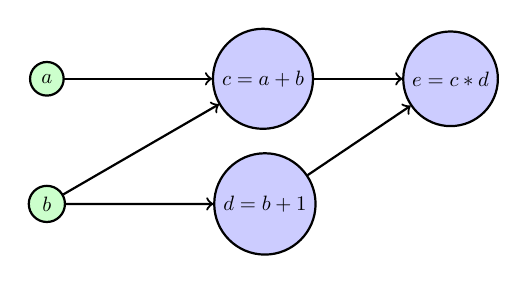
\begin{tikzpicture}[
    scale=0.75,         % <── overall scale factor
    every node/.style={transform shape}, % also resize node shapes & fonts
    node distance=2.5cm,
    op_node/.style={circle, draw, thick, fill=blue!20},
    var_node/.style={circle, draw, thick, fill=green!20}
    ]
    % Nodes
    \node[var_node] (a) {$a$};
    \node[var_node] (b) [below=1.5cm of a] {$b$};
    \node[op_node] (c) [right=of a] {$c=a+b$};
    \node[op_node] (d) [right=of b] {$d=b+1$};
    \node[op_node] (e) [right=1.5cm of c] {$e=c*d$};

    % Arrows
    \draw[->, thick] (a) -- (c);
    \draw[->, thick] (b) -- (c);
    \draw[->, thick] (b) -- (d);
    \draw[->, thick] (c) -- (e);
    \draw[->, thick] (d) -- (e);
\end{tikzpicture}
\end{center}

\textbf{Key Idea:} Any complex function, including a neural network, can be represented as a computational graph of simple, local operations.

\end{frame}
%==================================================================

%==================================================================
\begin{frame}
\frametitle{Forward Pass: Evaluating the Graph}

We can evaluate the expression by setting input values and computing nodes from left to right.
Let's set $a=2$ and $b=1$:

\begin{center}
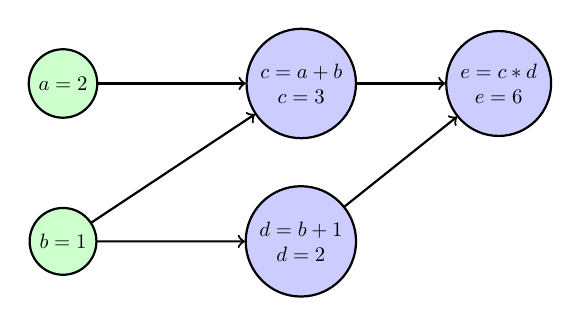
\begin{tikzpicture}[
    scale=0.75,                       % <── overall scale factor
    every node/.style={transform shape},
    node distance=2.5cm,
    op_node/.style={circle, draw, thick, fill=blue!20, align=center},
    var_node/.style={circle, draw, thick, fill=green!20, align=center}
    ]
    % Nodes
    \node[var_node] (a) {$a=2$};
    \node[var_node] (b) [below=1.5cm of a] {$b=1$};
    \node[op_node] (c) [right=of a] {$c=a+b$\\$c=3$};
    \node[op_node] (d) [right=of b] {$d=b+1$\\$d=2$};
    \node[op_node] (e) [right=1.5cm of c] {$e=c*d$\\$e=6$};

    % Arrows
    \draw[->, thick] (a) -- (c);
    \draw[->, thick] (b) -- (c);
    \draw[->, thick] (b) -- (d);
    \draw[->, thick] (c) -- (e);
    \draw[->, thick] (d) -- (e);
\end{tikzpicture}
\end{center}
This is exactly what a neural network's forward pass does: it computes layer by layer until it gets the final output (the cost).
\end{frame}
%==================================================================

%==================================================================
\begin{frame}
\frametitle{Derivatives on the Graph: The Chain Rule}

Now, let's find $\frac{\partial e}{\partial a}$ and $\frac{\partial e}{\partial b}$. The chain rule is our tool.
Let's label the edges with their local partial derivatives.
\begin{itemize}
    \item $\frac{\partial c}{\partial a} = 1$
    \item $\frac{\partial c}{\partial b} = 1$
    \item $\frac{\partial d}{\partial b} = 1$
    \item $\frac{\partial e}{\partial c} = d = 2$
    \item $\frac{\partial e}{\partial d} = c = 3$
\end{itemize}

\begin{center}
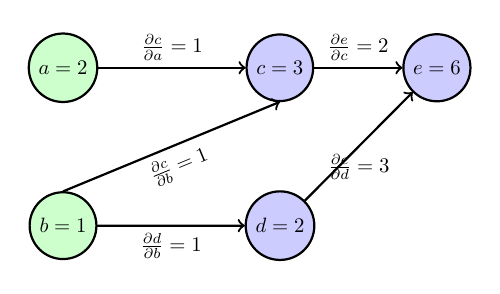
\begin{tikzpicture}[
    scale=0.75,                       % <── overall scale factor
    every node/.style={transform shape},
    node distance=2.5cm,
    op_node/.style={circle, draw, thick, fill=blue!20, align=center},
    var_node/.style={circle, draw, thick, fill=green!20, align=center}
    ]
    % Nodes (same as before)
    \node[var_node] (a) {$a=2$};
    \node[var_node] (b) [below=1.5cm of a] {$b=1$};
    \node[op_node] (c) [right=of a] {$c=3$};
    \node[op_node] (d) [right=of b] {$d=2$};
    \node[op_node] (e) [right=1.5cm of c] {$e=6$};
    
    % Arrows with derivatives
    \draw[->, thick] (a) -- (c) node[midway, above] {$\frac{\partial c}{\partial a}=1$};
    \draw[->, thick] (b.north) -- (c.south) node[midway, below, sloped] {$\frac{\partial c}{\partial b}=1$};
    \draw[->, thick] (b) -- (d) node[midway, below] {$\frac{\partial d}{\partial b}=1$};
    \draw[->, thick] (c) -- (e) node[midway, above] {$\frac{\partial e}{\partial c}=2$};
    \draw[->, thick] (d) -- (e) node[midway, below] {$\frac{\partial e}{\partial d}=3$};
\end{tikzpicture}
\end{center}

\textbf{The "Sum Over Paths" Rule:} To find the derivative of one node with respect to another, multiply the derivatives along every path between them and sum the results.
\begin{align*}
    \frac{\partial e}{\partial a} &= \frac{\partial e}{\partial c} \cdot \frac{\partial c}{\partial a} = 2 \cdot 1 = 2 \\
    \frac{\partial e}{\partial b} &= \underbrace{\frac{\partial e}{\partial c} \cdot \frac{\partial c}{\partial b}}_{\text{path via }c} + \underbrace{\frac{\partial e}{\partial d} \cdot \frac{\partial d}{\partial b}}_{\text{path via }d} = (2 \cdot 1) + (3 \cdot 1) = 5
\end{align*}
\end{frame}
%==================================================================

%==================================================================
\begin{frame}
\frametitle{The Problem: Combinatorial Explosion}

This "sum over paths" idea is mathematically correct, but computationally a disaster!
\begin{center}
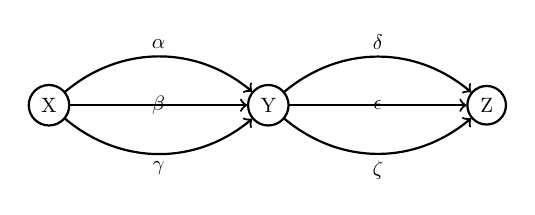
\begin{tikzpicture}[scale=0.75,
    every node/.style={transform shape}, node distance=3cm, auto]
    \node[circle, draw, thick] (X) {X};
    \node[circle, draw, thick] (Y) [right=of X] {Y};
    \node[circle, draw, thick] (Z) [right=of Y] {Z};
    \path[->, thick] (X) edge [bend left=40] node[above] {$\alpha$} (Y);
    \path[->, thick] (X) edge node {} (Y);
    \path[->, thick] (X) edge [bend right=40] node[below] {$\gamma$} (Y);
    \node at ($(X)!.5!(Y)$) {$\beta$};
    
    \path[->, thick] (Y) edge [bend left=40] node[above] {$\delta$} (Z);
    \path[->, thick] (Y) edge node {} (Z);
    \path[->, thick] (Y) edge [bend right=40] node[below] {$\zeta$} (Z);
    \node at ($(Y)!.5!(Z)$) {$\epsilon$};
\end{tikzpicture}
\end{center}
To get $\frac{\partial Z}{\partial X}$, we would need to sum $3 \times 3 = 9$ paths:
\begin{equation*}
    \frac{\partial Z}{\partial X} = \alpha\delta + \alpha\epsilon + \alpha\zeta + \beta\delta + \dots
\end{equation*}
In a deep neural network, the number of paths grows exponentially. We need a smarter way.

\textbf{The clever insight:} We can factor the sum!
\begin{equation*}
    \frac{\partial Z}{\partial X} = (\alpha + \beta + \gamma) \cdot (\delta + \epsilon + \zeta)
\end{equation*}
This is the core idea behind both Forward and Reverse-mode differentiation. They are just two different, efficient ways of computing this factored sum.

\end{frame}
%==================================================================

%==================================================================
\begin{frame}
\frametitle{Method 1: Forward-Mode Differentiation}

\textbf{Idea:} Start at an \textbf{input} and push derivatives forward. At each node, compute the derivative of \textit{that node} with respect to the chosen input.

Let's compute derivatives with respect to \textbf{a}: $\frac{\partial(\cdot)}{\partial a}$

\begin{center}
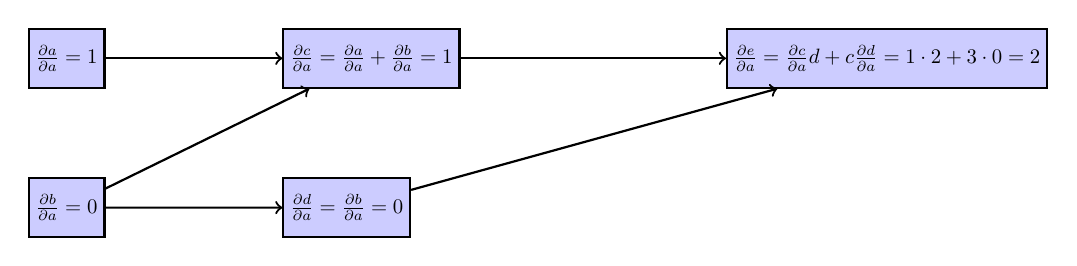
\begin{tikzpicture}[scale=0.75,every node/.style={transform shape},
    node distance=2.5cm and 1.5cm,
    op_node/.style={rectangle, draw, thick, fill=blue!20, align=center, minimum height=1cm},
    ]
    % Nodes
    \node[op_node] (a) {$\frac{\partial a}{\partial a} = 1$};
    \node[op_node] (b) [below=1.5cm of a] {$\frac{\partial b}{\partial a} = 0$};
    \node[op_node] (c) [right=3cm of a] {$\frac{\partial c}{\partial a} = \frac{\partial a}{\partial a} + \frac{\partial b}{\partial a} = 1$};
    \node[op_node] (d) [right=3cm of b] {$\frac{\partial d}{\partial a} = \frac{\partial b}{\partial a} = 0$};
    \node[op_node] (e) [right=4.5cm of c] {$\frac{\partial e}{\partial a} = \frac{\partial c}{\partial a}d + c\frac{\partial d}{\partial a} = 1\cdot2 + 3\cdot0 = 2$};

    % Arrows
    \draw[->, thick] (a) -- (c); \draw[->, thick] (b) -- (c);
    \draw[->, thick] (b) -- (d);
    \draw[->, thick] (c) -- (e); \draw[->, thick] (d) -- (e);
\end{tikzpicture}
\end{center}

\textbf{Result:} One forward pass gives us the derivative of the output with respect to \textbf{ONE} input.
\begin{equation*}
    \frac{\partial e}{\partial a} = 2
\end{equation*}

\textbf{Cost for a Neural Network:}
To get the gradient for all parameters, we would need to do one full forward pass for \textit{every single parameter}. If we have 1 million parameters, we need 1 million passes. Inefficient!

\end{frame}
%==================================================================

%==================================================================
\begin{frame}
\frametitle{Method 2: Reverse-Mode Differentiation (Backpropagation!)}

\textbf{Idea:} Start at the \textbf{output} and pull derivatives backward. At each node, compute the derivative of the \textit{final output} with respect to that node.

Let's compute derivatives with respect to every node: $\frac{\partial e}{\partial(\cdot)}$

\begin{center}
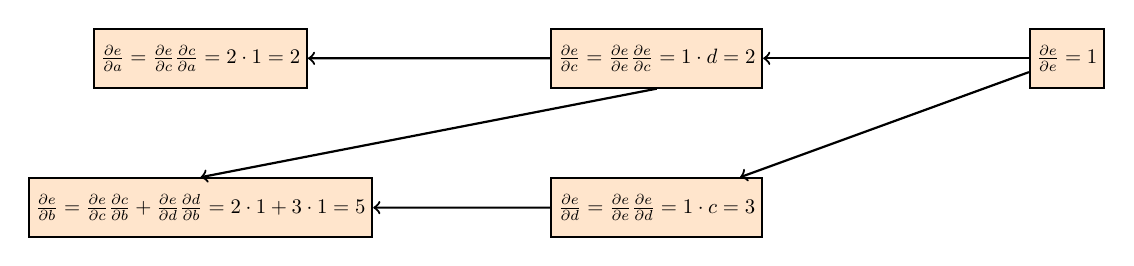
\begin{tikzpicture}[scale=0.75,every node/.style={transform shape},
    node distance=2.5cm and 1.5cm,
    op_node/.style={rectangle, draw, thick, fill=orange!20, align=center, minimum height=1cm},
    ]
    % Nodes
    \node[op_node] (e) {$\frac{\partial e}{\partial e} = 1$};
    \node[op_node] (c) [left=4.5cm of e] {$\frac{\partial e}{\partial c} = \frac{\partial e}{\partial e} \frac{\partial e}{\partial c} = 1 \cdot d = 2$};
    \node[op_node] (d) [below=1.5cm of c] {$\frac{\partial e}{\partial d} = \frac{\partial e}{\partial e} \frac{\partial e}{\partial d} = 1 \cdot c = 3$};
    \node[op_node] (b) [left=3cm of d] {$\frac{\partial e}{\partial b} = \frac{\partial e}{\partial c}\frac{\partial c}{\partial b} + \frac{\partial e}{\partial d}\frac{\partial d}{\partial b} = 2\cdot1 + 3\cdot1 = 5$};
    \node[op_node] (a) [above=1.5cm of b] {$\frac{\partial e}{\partial a} = \frac{\partial e}{\partial c}\frac{\partial c}{\partial a} = 2\cdot1 = 2$};

    % Arrows (reversed logic)
    \draw[<-, thick] (a) -- (c); \draw[<-, thick] (b.north) -- (c.south);
    \draw[<-, thick] (b) -- (d);
    \draw[<-, thick] (c) -- (e); \draw[<-, thick] (d) -- (e);
\end{tikzpicture}
\end{center}

\textbf{Result:} One reverse pass gives us the derivative of the output with respect to \textbf{ALL} inputs (and all intermediate nodes).
\begin{equation*}
    \frac{\partial e}{\partial a} = 2 \quad \text{and} \quad \frac{\partial e}{\partial b} = 5
\end{equation*}
\end{frame}
%==================================================================

%==================================================================
\begin{frame}
\frametitle{The Computational Victory: Why Reverse-Mode Wins}

Let's compare for a typical neural network:

\begin{columns}
\begin{column}{0.5\textwidth}
    \textbf{Forward-Mode}
    \begin{itemize}
        \item \textbf{Input:} Many (millions of parameters $w, b$)
        \item \textbf{Output:} One (the cost function $C$)
        \item One pass gives you $\frac{\partial C}{\partial w_1}$.
        \item To get the full gradient $\nabla C$, you need \textbf{millions of passes}.
    \end{itemize}
    \vspace{1cm}
    \textbf{Extremely inefficient!}\\
    (Like a model taking 200,000 years to train)
\end{column}
\begin{column}{0.5\textwidth}
    \textbf{Reverse-Mode (Backpropagation)}
    \begin{itemize}
        \item \textbf{Input:} Many (millions of parameters $w, b$)
        \item \textbf{Output:} One (the cost function $C$)
        \item One pass (plus one initial forward pass) gives you $\frac{\partial C}{\partial w_i}$ for \textbf{ALL $i$}.
        \item You get the full gradient $\nabla C$ in \textbf{one go}.
    \end{itemize}
    \vspace{1cm}
    \textbf{Massively efficient!}\\
    (Like a model taking a week to train)
\end{column}
\end{columns}

\vspace{1cm}
\textbf{Conclusion:} Backpropagation is not a new kind of calculus. It's just a very clever way of organizing the chain rule to be computationally efficient for the specific structure of neural networks (many inputs, one output).

\end{frame}
%==================================================================


%==================================================================
\begin{frame}
\frametitle{The Backpropagation Algorithm (The Four Equations)}

Now we can formalize this reverse-mode process for a feedforward network. We need four key equations.

\textbf{Notation:} $\delta^{(l)}_j$ is the "error" of neuron $j$ in layer $l$. It's a proxy for $\frac{\partial C}{\partial z^{(l)}_j}$.

\vspace{0.5cm}

\textbf{1. Output Layer Error ($\delta^{(L)}$):}
\begin{equation*}
    \delta^{(L)}_j = \frac{\partial C}{\partial a^{(L)}_j} \odot \sigma'(z^{(L)}_j) \quad \text{(BP1)}
\end{equation*}
How much the cost changes with respect to the output, scaled by how sensitive the activation function is.

\textbf{2. Hidden Layer Error ($\delta^{(l)}$):}
\begin{equation*}
    \delta^{(l)}_j = \left( \sum_k w^{(l+1)}_{kj} \delta^{(l+1)}_k \right) \odot \sigma'(z^{(l)}_j) \quad \text{(BP2)}
\end{equation*}
The error from the next layer is propagated back through the weights.

\textbf{3. Gradient for Biases ($\partial C / \partial b$):}
\begin{equation*}
    \frac{\partial C}{\partial b^{(l)}_j} = \delta^{(l)}_j \quad \text{(BP3)}
\end{equation*}
The gradient for a bias is simply the error of its neuron.

\textbf{4. Gradient for Weights ($\partial C / \partial w$):}
\begin{equation*}
    \frac{\partial C}{\partial w^{(l)}_{jk}} = a^{(l-1)}_k \delta^{(l)}_j \quad \text{(BP4)}
\end{equation*}
The gradient for a weight is the activation of the input neuron times the error of the output neuron.
\end{frame}
%==================================================================

%==================================================================
\begin{frame}
\frametitle{The Algorithm in Practice}

Here is the complete algorithm for one batch of data:

\begin{enumerate}
    \item \textbf{Input:} Set the input activation $a^{(1)}$.
    
    \item \textbf{Forward Pass:} For each layer $l = 2, 3, \ldots, L$:
    \begin{itemize}
        \item Compute $z^{(l)} = W^{(l)}a^{(l-1)} + b^{(l)}$
        \item Compute $a^{(l)} = \sigma(z^{(l)})$
        \item Store all $z^{(l)}$ and $a^{(l)}$ values.
    \end{itemize}
    
    \item \textbf{Backward Pass (The Core of Backprop):}
    \begin{itemize}
        \item \textbf{Output Error:} Compute $\delta^{(L)}$ using (BP1).
        \item \textbf{Propagate Error:} For each layer $l = L-1, L-2, \ldots, 2$:
        \begin{itemize}
            \item In matrix form: $\delta^{(l)} = ((W^{(l+1)})^T \delta^{(l+1)}) \odot \sigma'(z^{(l)})$ using (BP2).
        \end{itemize}
    \end{itemize}
    
    \item \textbf{Gradient Computation:} For each layer $l = L, L-1, \ldots, 2$:
    \begin{itemize}
        \item Compute $\frac{\partial C}{\partial b^{(l)}} = \delta^{(l)}$ using (BP3).
        \item Compute $\frac{\partial C}{\partial w^{(l)}} = \delta^{(l)} (a^{(l-1)})^T$ using (BP4).
    \end{itemize}
    
    \item \textbf{Update:} Use the computed gradients in your SGD step.
\end{enumerate}

\end{frame}
%==================================================================

%==================================================================
\begin{frame}
\frametitle{Conclusion: Key Takeaways}

\begin{enumerate}
    \item \textbf{Computational graphs} are a powerful way to think about complex functions and their derivatives.
    \vspace{0.5cm}
    \item Backpropagation \textbf{is not} a new type of calculus. It's an algorithm that cleverly applies the \textbf{chain rule} in reverse.
    \vspace{0.5cm}
    \item It is formally known as \textbf{reverse-mode automatic differentiation}.
    \vspace{0.5cm}
    \item Its incredible efficiency comes from the specific structure of neural network training: we want the derivatives of \textbf{one output} (the cost) with respect to \textbf{many inputs} (the parameters).
    \vspace{0.5cm}
    \item This single insight is what makes training deep models with millions of parameters computationally tractable and is the foundation of the entire deep learning revolution.
\end{enumerate}

\end{frame}
%==================================================================

\end{document}